\section{Expression analysis (tuxedo)}
There are several tools able to do differential gene expression analysis, like CuffDiff, EdgeR and DESeq2, all available for Galaxy. For this analysis we will start use CuffLinks and CuffDiff and use the data created in the alignment exercise. If you were not able to make ``HISAT2 on miR-23b.bam'' and `` HISAT2 on control sample.bam'', you can import them from the data library:\\
\datalibrarydirrnaseqtuxedo \\
Simetimes it can be handy to obtain some extra details from your BAM files, for example if they are given to you by a third party. Find the tool ``BAM-to-SAM" and select the following settings:\\
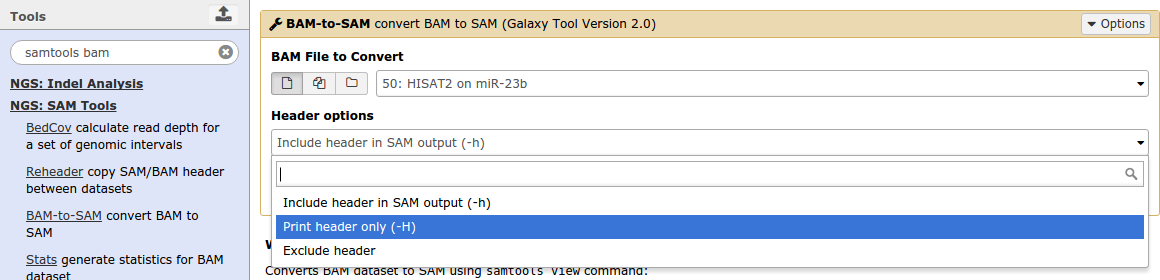
\includegraphics[width=\textwidth]{figures/basic_01.png}\\
\begin{itemize}
	\item Can you find out which version of which aligner (e.g. Tophat2, HISAT2 or RNA-STAR) was used?
\end{itemize}
As you might have seen when we visualized the alignments, it is not really feasible to find expression levels or determine genes by `eye'. To assemble the expressed genes and estimate the corresponding expression levels we will make use of the \textit{Tuxedo pipeline}. The program CuffLinks assembles genes, isoforms, measures gene expression and sets the basis for differential gene expression analysis. Run CuffLinks on both alignments separately:\\
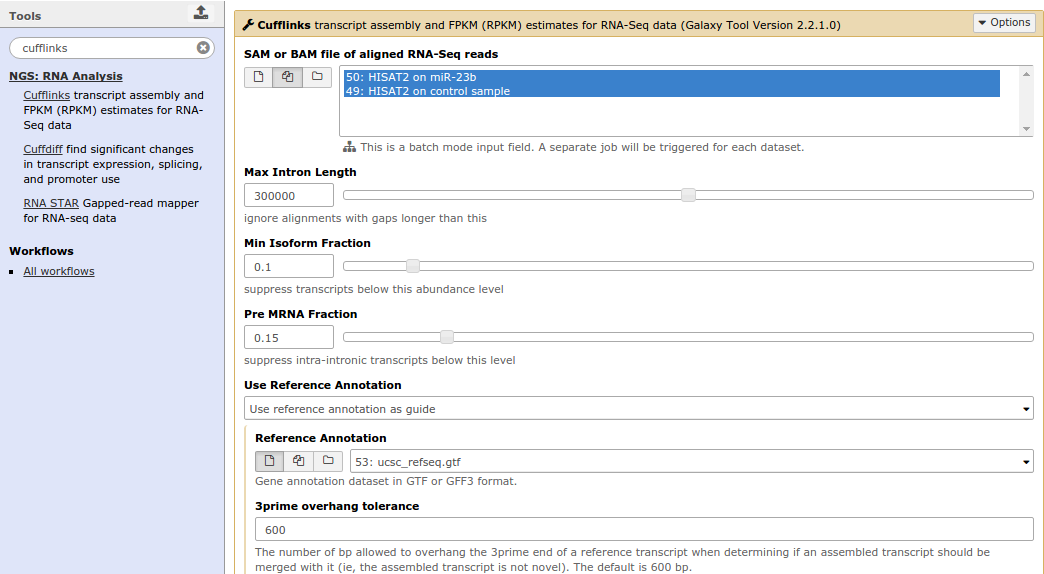
\includegraphics[width=\textwidth]{figures/basic_02a.png}\\
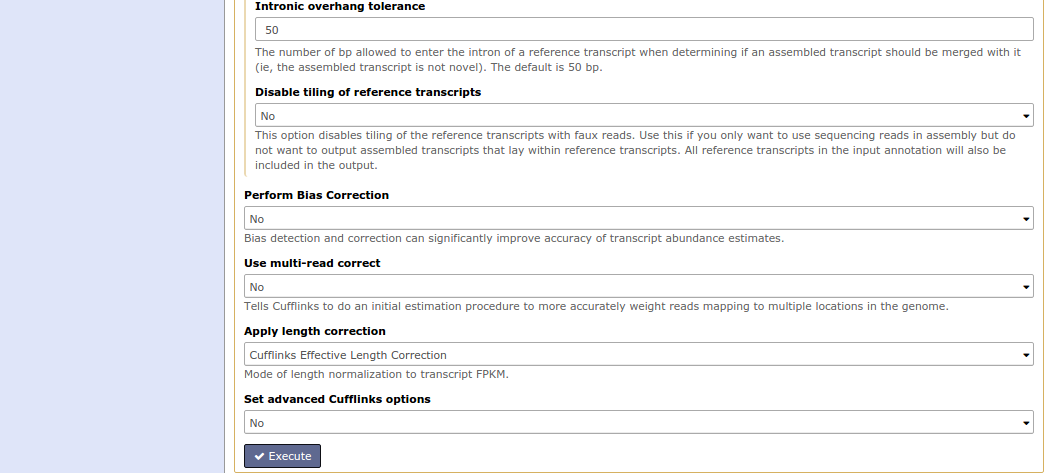
\includegraphics[width=\textwidth]{figures/basic_02b.png}\\
We have selected the \textit{Reference annotation} as guide, meaning that it uses a known gene annotation as basis for the assembled genes and adds possible new exons or genes to it. Because each sample may contain its own unique expressed transcripts, all assembled have to be merged into one transcript annotation before doing comparative expression analysis such that we can do analysis on the known (ucsc) and newly discovered transcripts:\\
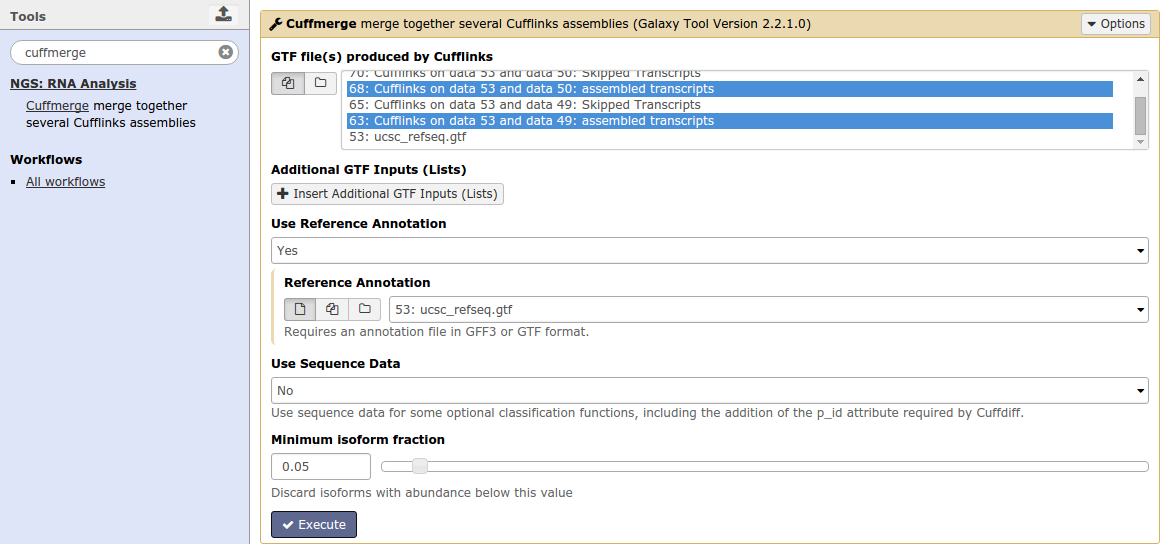
\includegraphics[width=\textwidth]{figures/basic_03.png}\\
To compare the expression profiles with each other, we use CuffDiff. Please note that we use only 1 replicate per condition which is statistically speaking a non-ideal setup. Therefore we need to set the dispersion estimation method to \textit{blind}. Proceed with the following settings and leave the rest default:\\
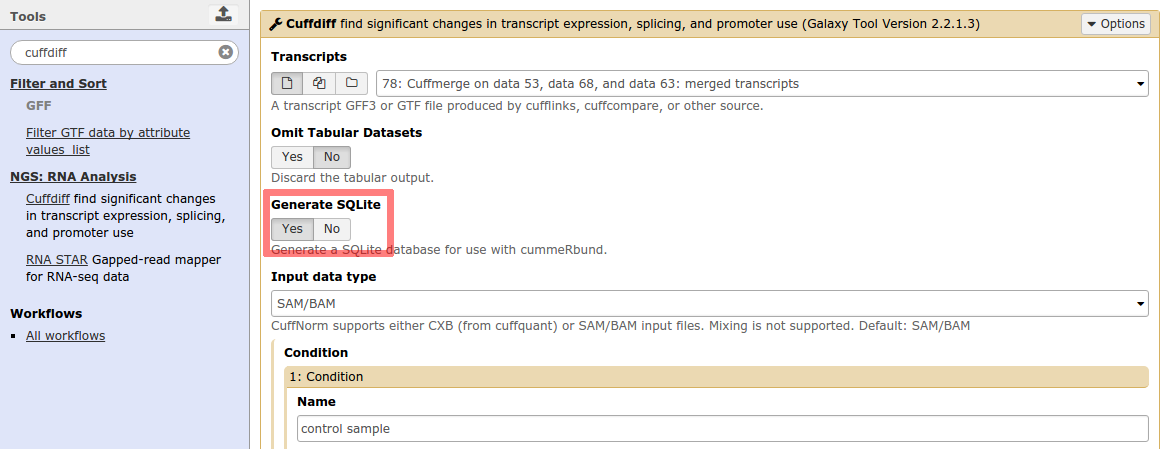
\includegraphics[width=\textwidth]{figures/basic_04a.png}\\
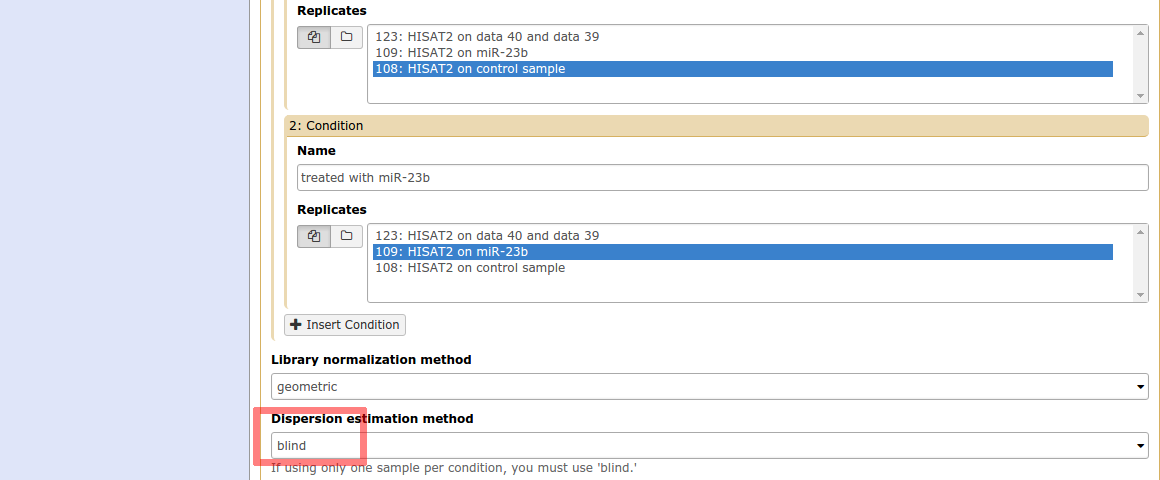
\includegraphics[width=\textwidth]{figures/basic_04b.png}\\
This analysis will create a bunch of new history items for different tests that are being applied. Look carefully before selecting the file to answer the following question:
\begin{itemize}
	\item What is the most differentially expressed gene between the sample treated with miR-23b and its control?
	\item Is there similarity with the significant genes detected in:\\\url{https://www.ncbi.nlm.nih.gov/pmc/articles/PMC3664824/figure/gkt245-F6/}
\end{itemize}
Except for CummeRbund, we have now gone through all steps of the Tuxedo pipeline individually.
